\documentclass[12pt,letterpaper]{article}
\usepackage{fullpage}
\usepackage[top=2cm, bottom=4.5cm, left=2.5cm, right=2.5cm]{geometry}
\usepackage{amsmath,amsthm,amsfonts,amssymb,amscd}
\usepackage{lastpage}
\usepackage{enumerate}
\usepackage{fancyhdr}
\usepackage{mathrsfs}
\usepackage{xcolor}
\usepackage{graphicx}
\usepackage{listings}
\usepackage{hyperref}
\usepackage{graphicx}
\usepackage{tikz}

\hypersetup{%
  colorlinks=true,
  linkcolor=blue,
  linkbordercolor={0 0 1}
}
 
\renewcommand\lstlistingname{Algorithm}
\renewcommand\lstlistlistingname{Algorithms}
\def\lstlistingautorefname{Alg.}

\lstdefinestyle{Python}{
    language        = Python,
    frame           = lines, 
    basicstyle      = \footnotesize,
    keywordstyle    = \color{blue},
    stringstyle     = \color{green},
    commentstyle    = \color{red}\ttfamily
}

\setlength{\parindent}{0.0in}
\setlength{\parskip}{0.05in}

% Edit these as appropriate
\newcommand\course{CSE 3500}
\newcommand\hwnumber{0}                  % <-- homework number
\newcommand\NetIDa{bec19009}           % <-- NetID of person #1

\pagestyle{fancyplain}
\headheight 35pt
\lhead{\NetIDa}
\chead{\textbf{\Large Homework \hwnumber}}
\rhead{\course \\ \today}
\lfoot{}
\cfoot{}
\rfoot{\small\thepage}
\headsep 1.5em

\begin{document}

\begin{center}
    \LARGE Problem Set
\end{center}
\begin{center}
    \textbf{Please be kind while grading :)}    
\end{center}


\section*{Problem 0 -- Collaboration Policy (10\%)}
Read and sign the Collaboration Policy in the Course Content folder on HuskyCT.
Hand in your signed form with your homework submission.
We cannot grade your work without a signed form.
\begin{center}
    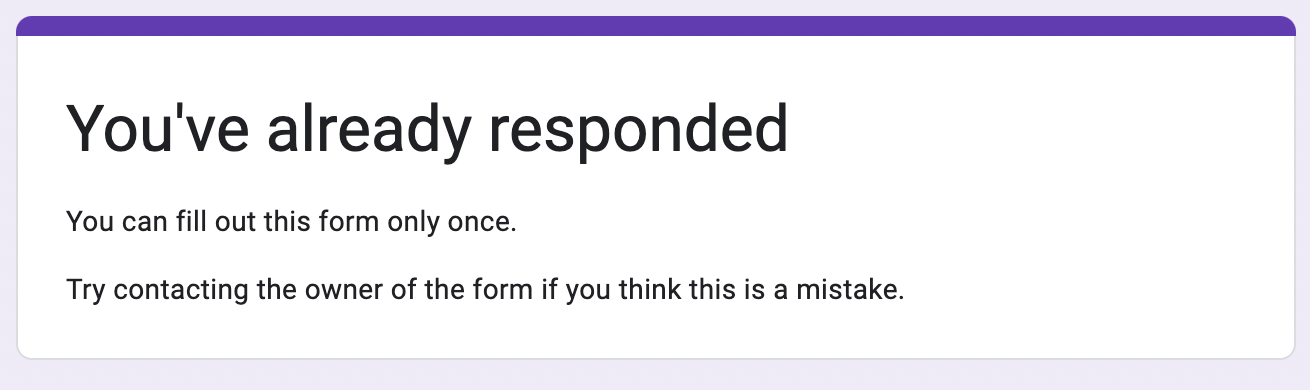
\includegraphics[scale=.7]{images/confirm.png}    
\end{center}


\section*{Problem 1 -- Introductions (10\%)}
The goal of this problem is to introduce yourself to the course staff and to think about what you want to get out of the course.
Write at most two paragraphs about yourself.
This may include your academic and non-academic interests, preferred programming languages, courses that you are excited to take in the future, or areas of computer science that you find the most interesting.
Finish by describing what do you want to learn by taking this course.
Think about what would be most beneficial to your prospective career.

\subsection*{Introduction:}
Hi my name is Benny and I am a Junior majoring in Computer Science. I mainly am taking this class
for my major however I know the importantance of learning Algorithms and Complexities in Computer Science 
so I want to learn as much as I can from this class. I currently am a Data Analytics concentration as 
I like looking at and manipulating data. I somewhat like algorithms however I am not the best at prooving them
like with complexities associated with them. I personally like programming in python as it is easy to use and 
verstile enough for smaller tasks, however I also like programming in C++. I am most intrested in machine learning
in the computer science field as I love the applications and possibilities of it. From this class my goal is to learn 
how to prove algorithms and their complexities as well as learn more about the different types of algorithms. 
\newpage

\section*{Problem 2 -- Preliminaries (10\%)}
This problem tests your retention of prerequisite materials.
If some of these problems are difficult, please go back and review material from the prerequisites.

\subsection*{Questions:}
\begin{enumerate}
    \item How many permutations are there of the set of $n$ numbers? 
    \item How many subsets of three numbers are there from a set of $n$ numbers?
    \item How many subsets of $S$ are there when $|S|=n$?
\end{enumerate}

\subsection*{Answer:}
\begin{enumerate}
    \item Of a set of $n$ numbers, there are going to be $n!$ permutations. 
    As there are $n$ numbers, there are $n$ ways to choose the first number, 
    $n-1$ ways to choose the second number, and so on. Each of these choices 
    is independent of the others, so the total number of permutations is the 
    product of the number of choices for each position. 
    \item There are going to be $n^3$ subsets of three numbers from a set of $n$ numbers.
    \item There are going to be $2^n$ subsets of $S$ when $|S|=n$.
\end{enumerate}

\newpage

\section*{Problem 3 -- Complexity (20\%)}

\begin{enumerate}
    \item For functions $A$ and $B$ and constant $c>1$, indicate which of $\{A = O(B),A = \Omega(B),A = \Theta(B)\}$ holds. Here, we use the notation that $log_2=lg$. \textit{Hint: for these problems it is useful to know some mathematical identities. See CLRS section 3.2 or \textbf{standard\_notations\_and\_common\_functions.pdf} in HuskyCT Lecture 2 course notes.} 
    \begin{enumerate}
        \item $A=n^c$, $B=c^n$
        \item $A=n^{lg(c)}$, $B=c^{lg(n)}$
        \item $A=lg(n!)$, $B=lg(n^n)$. For this problem, you will find Stirling's approximation useful: $n!=\sqrt{2 \pi n}\left( \frac{n}{e} \right)^n \left( 1 + \Omega \left( \frac{1}{n} \right) \right)$.
        \item $A=3^{3^n}$, $B=3^{n^2}$
    \end{enumerate}
    \item Place the following functions in increasing order of growth rate. I.e. if $g$ follows $f$ then $f=O(g)$ is true.
    \begin{enumerate}
        \item $n^e$, 
        \item $n^{\lg(n)}$
        \item $n^\pi$, 
        \item $\lg(n!)$
        \item $2^{\sqrt{\lg(n)}}$
        \item $n$
    \end{enumerate}
\end{enumerate}

\subsection*{Answer:}
\begin{enumerate}
    \item \begin{enumerate}
        \item $A = O(B)$
        \item $A = \Theta(B)$
        \item $A = O(B)$
        \item $A = \Omega(B)$
    \end{enumerate}
    \item \begin{enumerate}
        \item $2^{\sqrt{\lg(n)}}$
        \item $n$
        \item $\lg(n!)$
        \item $n^e$
        \item $n^\pi$
        \item $n^{\lg(n)}$
    \end{enumerate}

\end{enumerate}


\newpage

\section*{Problem 4 --  Vinder (30\%)}
Vinder is a new smartphone app designed to make it easier for everyone to eat their vegetables. 
Vinder compares your genetic information with a large database of vegetable genetic sequences to match you with the right vegetable based on sequence similarity. 
Specifically, it computes the longest common subsequence between your DNA sequence and the DNA sequences of thousands of vegetables. 

An $n$-length \textit{DNA sequence}, $A$, is an ordered collection of elements $\in [A,C,G,T]$, or $A\in[A,C,G,T]^n$.
A \textit{subsequence} is a sequence formed by deleting elements from another sequence, thus preserving the original order.
A $k$-length \textit{prefix} of sequence $A$ is the first $k$ elements of $A$.
For example, $A=[A,C,C,G,G,A,A,T,C]$ is a sequence. $[A,C,A,T]$ and $[C]$ are subsequences of $A$ but $[T,A]$ is not. $[A,C,C,G]$ is a $4$-prefix of $A$ and $[ ]$ is the $0$-prefix.

Our goal is to find the longest common subsequence (LCS) of $A$, the human DNA sequence, and sequences $B^k \in D$ where $D$ is the database of vegetable DNA sequences and $k=1,...,|D|$.
This solution can be found efficiently using dynamic programming. 
At a high-level, the algorithm is:
\begin{enumerate}
    \item For each sequence $B^k\in D$
    \item Initialize the length of the LCS to $0$.
    \item Let $A_i$ denote the $i^{th}$ element of $A$. 
    Consider each pair of $A_i$ and $B^k_j$; either $A_i=B^k_j$ or $A_i \neq B^k_j$.
    \begin{itemize}
        \item If $A_i=B^k_j$, then the length of the LCS of the $i$-prefix of $A$ and $j$-prefix of $B^k$ is one more than the LCS of the $i-1$-prefix of $A$ and $j-1$-prefix of $B^k$.
        \item If $A_i \neq B^k_j$, then we cannot extend the LCS. 
        Instead, we conclude that the LCS up to $(A_i,B^k_j)$ is the maximum of the LCS up to $(A_{i-1},B^k_j)$ or $(A_i,B^k_{j-1})$.
    \end{itemize}
\end{enumerate}
The two aforementioned cases sum up the possibilities at $(A_i,B^k_j)$.
We can use these to recursively define the LCS in terms of smaller problem solutions.
Your goal is to describe the algorithm to do this.
\begin{enumerate}
    \item Describe an algorithm to find the length of the LCS that does not use dynamic programming. 
    You do not have to write pseudocode, simply describe the algorithm in enough detail so that we understand it. 
    What is the runtime?
    Why is it correct?
    You may keep your answers informal. 
    \textit{Hint: a brute-force  or recursive solution should have exponential runtime.}
    \vspace{0.5cm}

    \textbf{Answer:}
    A algorithm that does not use dynamic programming to solve this problem would be to try all possible subsequences of $A$ and $B^k$ and find the longest one. 
    We can do this by checking if the first element of $A$ is the same as the first element of $B^k$ and if it is, we can check the rest of the subsequences of 
    $A$ and $B^k$ by removing the first element of both sequences. 
    This would have exponential runtime because there are $2^n$ possible subsequences of $A$ and $2^m$ 
    possible subsequences of $B^k$ where $n$ and $m$ are the lengths of $A$ and $B^k$ respectively. This would be a brute force solution and would not be efficient.
    \vspace{0.5cm}
    
    \item Write out the recurrence relation used in the algorithm defined in the problems description (not part 1 of the answers). 
    That is, write out how the LCS length can be expressed in terms of smaller instances of the problem.
    \vspace{0.5cm}

    \textbf{Answer:}
    Let $LCS(i,j)$ be the length of the LCS of the $i$-prefix of $A$ and $j$-prefix of $B^k$. 
    Then, $LCS(i,j) = \begin{cases}
        0 & \text{if } i=0 \text{ or } j=0 \\
        LCS(i-1,j-1)+1 & \text{if } A_i=B^k_j \\
        \max(LCS(i-1,j),LCS(i,j-1)) & \text{if } A_i \neq B^k_j
    \end{cases}$

    \item Think about how to convert this into a dynamic program. What size table would you need for the LCS problem?
    \vspace{0.5cm}

    \textbf{Answer:}
    We would need a table of size $n\times m$ where $n$ is the length of $A$ and $m$ is the length of $B^k$. 

    \item Interpret each table entry. That is, give your explanation for what each entry in the dynamic programming table represents. 
    We discussed how to interpret the entries of the dynamic programming table for the similar problem of \textit{edit distance}.
    \vspace{0.5cm}

    \textbf{Answer:}
    Each entry in the table represents the length of the LCS of the $i$-prefix of $A$ and $j$-prefix of $B^k$. 
    \vspace{4in}

    \item Write out the table for $Derek: [A,C,A,G,G,T,T,A,C]$ and\\
    $Asparagus\footnote{provably the best vegetable}: [T,C,G,G,A,A,T,A,A]$.
    \vspace{0.5cm}

    \textbf{Answer:}
    \begin{center}
        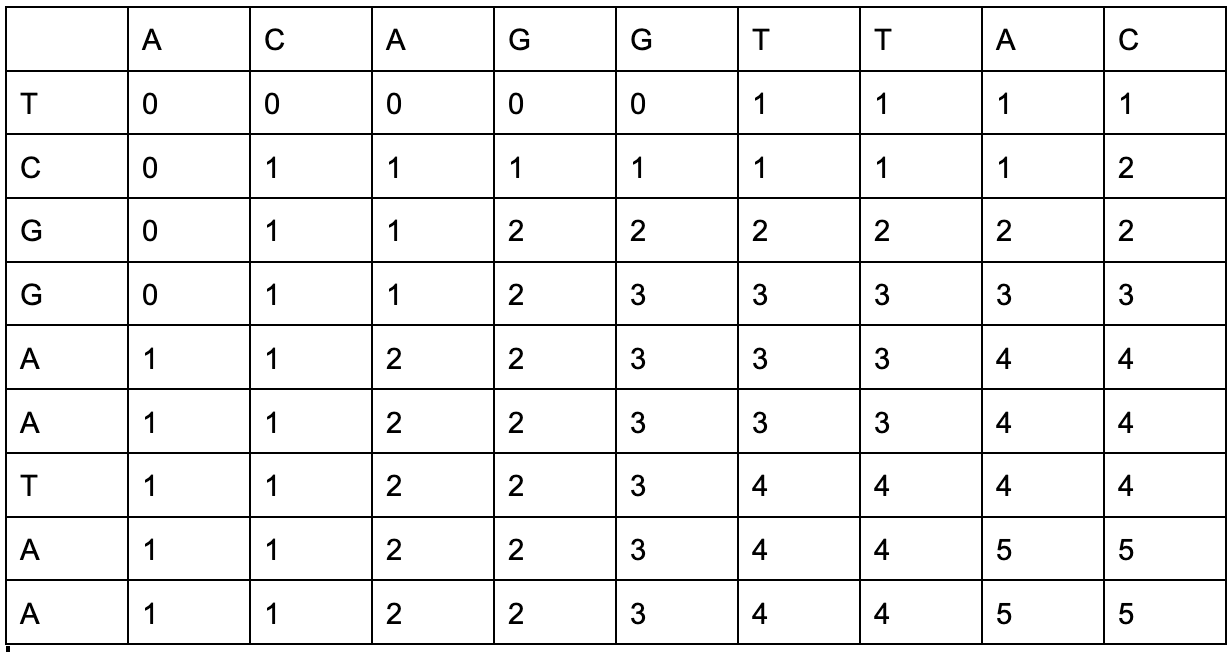
\includegraphics[scale = .7]{images/table.png}
    \end{center}
    
        \newpage

    \item Prove your LCS algorithm's (that you defined in 2-5) correctness. 
    \textit{Hint: Many dynamic programming proofs follow a simple structure. Consider the following template:}
    \begin{enumerate}
        \item Describe what you will show. This should include the variables used to index the table, presented in the order in which your algorithm fills the table values. 
        Also detail here what your algorithm is supposed to compute.
        \item State your induction hypothesis. 
        This includes stating your base case and how your algorithm correctly computes the base cases.
        Then describe an arbitrary input and corresponding arbitrary entry in the table that will be computed. You can think of this as a \textit{state} of the algorithm at one particular time point.
        Next, consider an optimal dynamic programming table for your particular problem; detail the last decision made in this optimal solution. This usually falls under a number of different cases based on your recurrence relation.
        \item Consider each case; assuming that everything in the dynamic programming table is correct, prove that your algorithm will correctly compute the current entry in the table.
        Show that your recurrence relation accurately describes each possibility for the last choice made by the unknown LCS.
        This is the part of your proof where you compare the real world possibilities to the cases in your code.
        By showing this, your recurrence relation and code rely on the previous entries in the table to produce a solution at least as good as the optimal LCS.
    \end{enumerate}
    \vspace{0.5cm}

    \textbf{Answer:}
    \begin{enumerate}
        \item We will show that the algorithm correctly computes the length of the LCS of $A$ and $B^k$.
        The algorithm will fill the table in a bottom-up fashion. It will fill the first row and column with 0's. 
        Then, it will fill the rest of the table by considering the case where $A_i=B^k_j$ and the case where $A_i \neq B^k_j$.
        In the case where $A_i=B^k_j$, the algorithm will fill the table entry with the value of the table entry in the previous row and column plus 1. 
        \item Our induction hypothesis is that the algorithm correctly computes the length of the LCS of the $i$-prefix of $A$ and $j$-prefix of $B^k$ for all $i,j$.
        \item The algorithm will correctly compute the length of the LCS of the $i$-prefix of $A$ and $j$-prefix of $B^k$ by taking the maximum of the length of the LCS of the $(i-1)$-prefix of $A$ and $j$-prefix of $B^k$ and the length of the LCS of the $i$-prefix of $A$ and $(j-1)$-prefix of $B^k$.
        This is because the algorithm will correctly compute the length of the LCS of the $(i-1)$-prefix of $A$ and $j$-prefix of $B^k$ and the length oAf the LCS of the $i$-prefix of $A$ and $(j-1)$-prefix of $B^k$ by the induction hypothesis.
        The base case is that the algorithm correctly computes the length of the LCS of the $0$-prefix of $A$ and $0$-prefix of $B^k$ which is 0. In this case, the algorithm will correctly compute the length of the LCS of the $i$-prefix of $A$ and $j$-prefix of $B^k$ by the induction hypothesis. 
        In the case where $A_i=B^k_j$, the algorithm will correctly compute the length of the LCS of the $i$-prefix of $A$ and $j$-prefix of $B^k$ by taking the value of the table entry in the previous row and column plus 1. 



    \end{enumerate}
    
\end{enumerate}

\newpage

\newpage


\section*{Problem 5 -- Longest Path Problem (20\%)}
We are given a directed, unweighted graph $G=(V,E)$ where $v_i \in V$ for $i=1,...,n$.
Additionally, $G$ is ordered, meaning
\begin{itemize}
    \item An edge can only originate from a vertex with lower index than its destination. Formally, edges may only have the form $(v_i,v_j)$ where $i<j$.
    \item The only \textit{absorbing} node is $v_n$. Absorbing nodes have out-degree $0$.
\end{itemize}

Given an ordered, unweighted, directed graph $G(V,E)$, the \textit{longest path problem} is to compute the longest path length from $v_1$ to $v_n$.

    \lstset{caption={Longest path algorithm}}
    \lstset{label={lst:alg1}}
    \begin{lstlisting}[style = Python]
    def longest_path(v1):
        iter=v1
        length=0
        while iter.hasOutgoingEdge():
            iter=iter.getEdgeSmallestIndex()
            length+=1
        return length
            
    \end{lstlisting}

\begin{enumerate}
    \item Demonstrate that Alg. \ref{lst:alg1} does not correctly solve the problem by giving a counter-example as a graph. 
    The function \texttt{iter.hasOutgoingEdge()} returns a boolean indicating whether or not the vertex \texttt{iter} has an outgoing edge.
    The function \\
    \texttt{iter.getEdgeSmallestIndex()} returns the smallest index of all vertices incident from \texttt{iter}. 
    That is, $min_j \{ (iter,v_j) \in E \}$.
    We prefer that your solution be a graph embedding either by hand-drawing and scanning or taking a picture, or drawing it digitally. 
    If none of these options are available, you can simply list the set of edges in the graph.
    \vspace{0.5cm}

    \textbf{Answer:}
    \begin{center}
        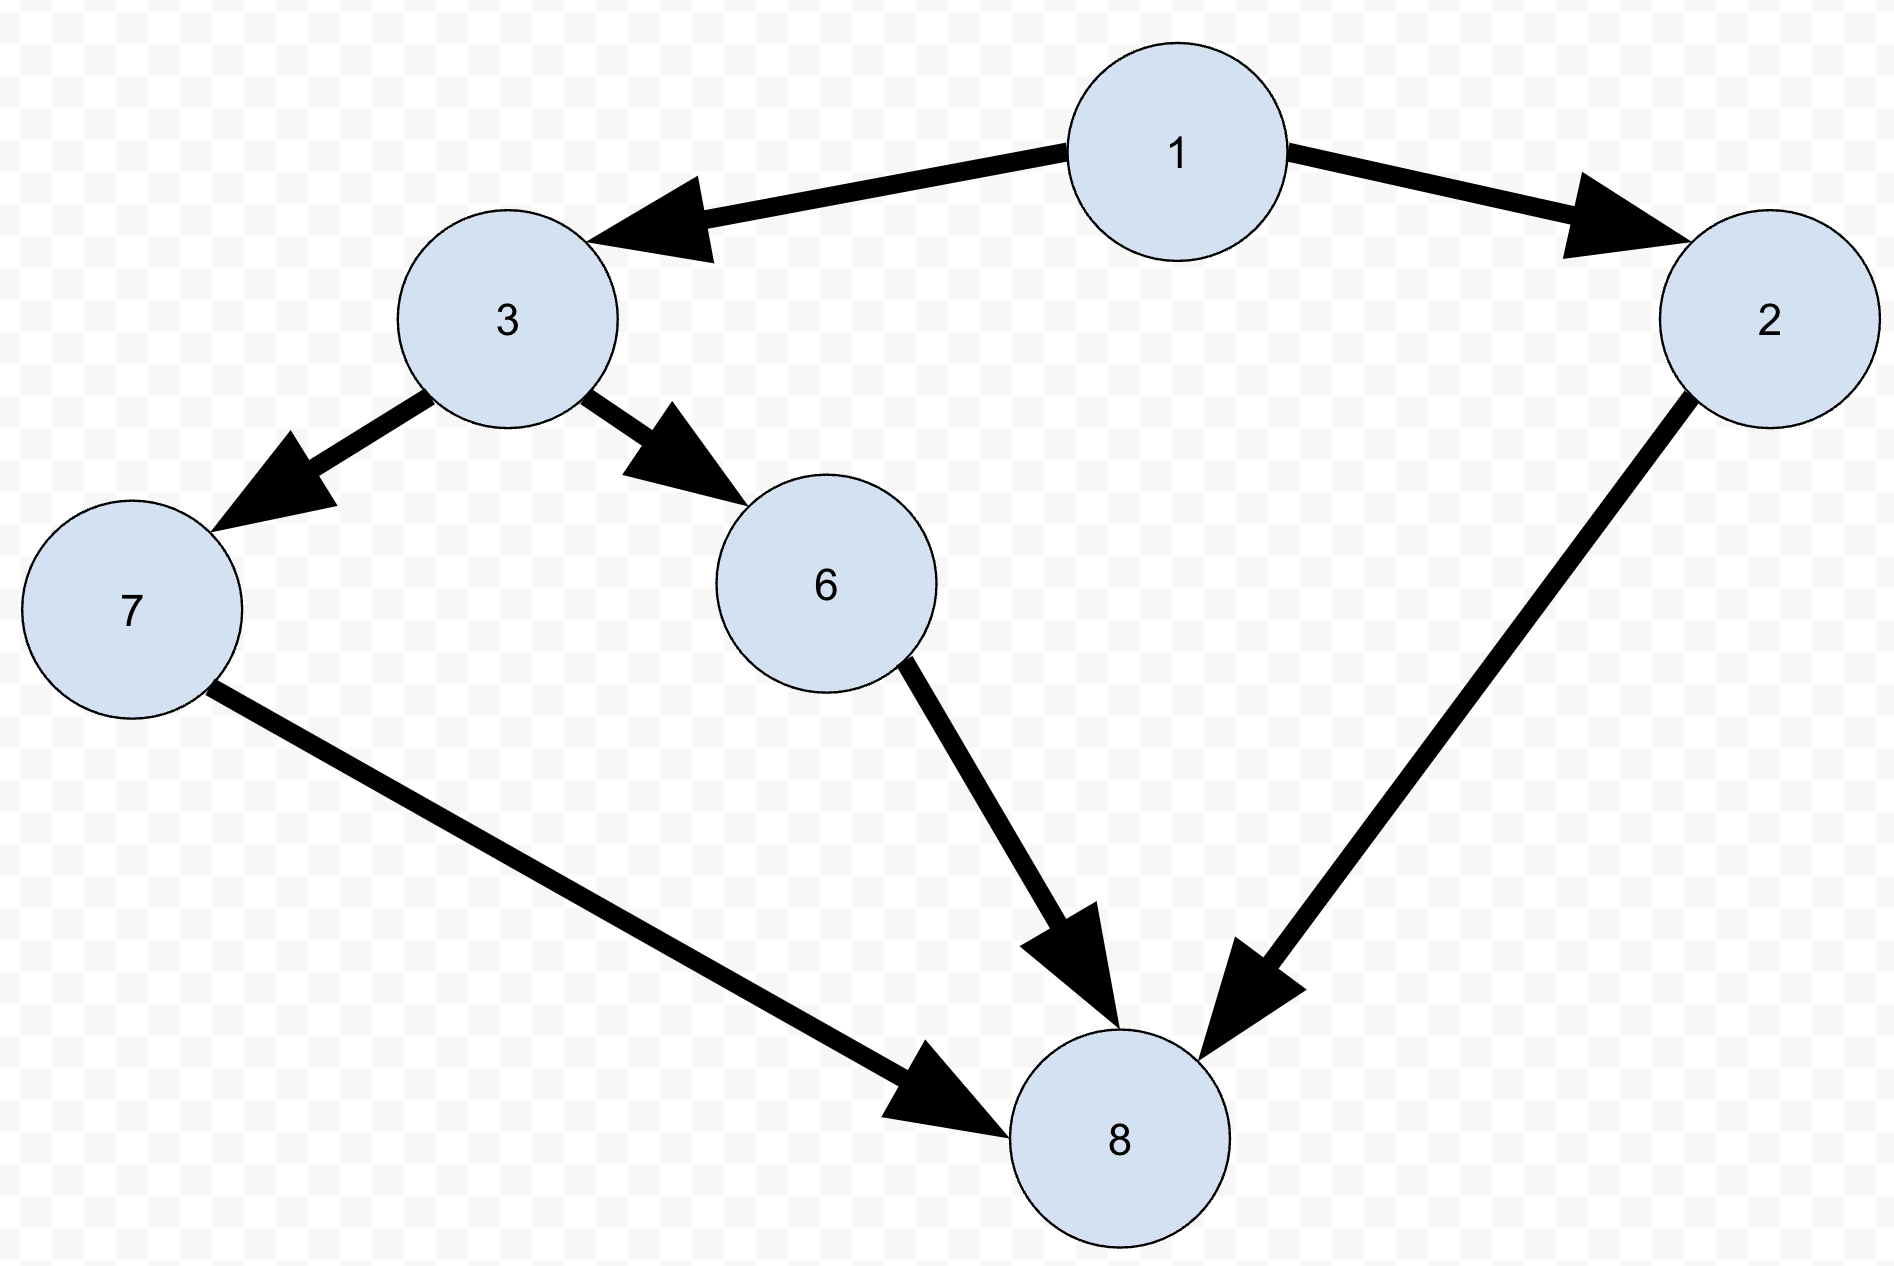
\includegraphics[scale = .25]{images/graph.png}
    \end{center}
        \newpage

    \item Develop an $O(n^2)$ algorithm for solving the  \textit{longest path problem} in ordered, unweighted, directed graphs. 
    Besides the functions defined above, you are free to use any function associated with graph data structure implementations.
    \vspace{0.5cm}

    \textbf{Answer:}
    \begin{lstlisting}[style = Python]
    def longest_path(v1):
        length=0
        for node in v1:
            path=[node]
            while node.hasOutgoingEdge():
                node=node.getEdgeSmallestIndex()
                path.append(node)
            if len(path)>length:
                length=len(path)

        return length

    \end{lstlisting}
    
    
\end{enumerate}

\end{document}
